\chapter{Teoretiskt ramverk}

I detta avsnitt presenteras härledningar av de fysikaliska fenomen och beräkningsmetoder projektet baseras på samt definitioner av, för projektet, centrala begrepp. För full förståelse krävs en viss matematisk bakgrund, men i många fall kan läsaren helt hoppa över härledningarna. 
% Konventioner listas efter denna kommentar...
% Följande kanske inte behövs, vilken nivå ska vi förvänta oss av en läsare?
% Nabla- ($\nabla$) och Laplaceoperatorn ($\Delta$) kommer på sina ställen att användas i ekvationerna. Dessa betecknar vektorerna $\left( \frac{\partial}{\partial x}, \frac{\partial}{\partial y}, \frac{\partial}{\partial z}\right)$ respektive $\left( \frac{\partial^2}{\partial x^2}, \frac{\partial^2}{\partial y^2}, \frac{\partial^2}{\partial z^2} \right)$. Gradienten av skalären $T$ blir då $\nabla T = \left( \frac{\partial T}{\partial x}, \frac{\partial T}{\partial y}, \frac{\partial T}{\partial z}\right)$. 

\section{Definition av väder för tillämpningar i denna rapport}
\label{subsec_weather}
Vår uppdragsgivare vill undersöka hur inomhustemperaturen påverkas av vädret. Tesen är att man kan få en mer korrekt styrning av inomhustemperaturen om man inte bara låter den påverkas av utomhustemperaturen, utan även av fler väderparamterar. Han har därför installerat en väderstation, se avnitt~ \ref{subsec_weathertransmitter}.

Begreppet väders vardagliga användningsområde är mycket brett och behöver därför avgränsas för att definiera de väderparameterar som behandlas inom projektet.

Kortfattat definieras vädret som det väderstation tillsammans med solintensitetsmätaren mäter. Så som finns beskrivet i avsnitt~\ref{subsec_weathertransmitter} mäter vi vädret med utrustning som tar in vindens hastighet och riktning, lufttemperaturen, lufttryck, relativ fuktighet samt regn och hagels varaktighet och intensitet. Vi kommer dock att bortse helt ifrån hagel då detta sker så sällan och i så korta perioder att det kan antas försumbart.  Dessutom mäter solintensitetsmätaren solens intensitet och varaktighet, se avsnitt~\ref{subsec:sunmeter}. % Källa på hur ofta (sällan) det haglar i Sverige. 

Tanken är att man ska kunna beskriva allt väder som en temperatur, antingen som den utomhustemperatur man bör reglera efter eller som den inomhustemperatur huset skulle få med befintlig aktivitet men utan uppvärmning, alltså ett mått på hur många grader man måste värma. Dessa två mått kallas ekvivalent temperatur och free-running temperature vilka beskrivs i avsnitt~\ref{sec:ekv_temp} respektive avsnitt~\ref{sec:freerunningtemp}. 

Från studier med hjälp av beräkningstjänsten Wolfram Alpha\cite{wolframalpha} av hur luftfuktighet kan påverkar luftens värmeledningsförmåga, får vi att den har väldigt liten betydelse. Man kan se en liten skillnad vid mycket höga luftfuktigheter (upp emot 90 \%) vid de högre temperaturerna, över $\unit[25]{^\circ C}$. Detta torde vara försumbart eftersom skillnaden är liten och endast vid väderförhållanden som inträffar relativt sällan i vårt klimat.

Hur regn och fukt påverkar fastighetensklimat har inte behandlats inom det här projektet.
Det kan dock antas att en hel del energi försvinner när väggen blir blöt och vattnet avdunstar. Troligen kyler regnet även luften.

Ytterligare en parameter som inte behandlas till är snö. När snön har lagt sig på taket kan man anta att den har en isolerande effekt. Vi kan inte mäta om och i så fall hur mycket snö det ligger på taket. Enligt SMHI\cite{SMHIdata}
rör det sig enbart om 25-50 dygn med snö i Göteborg per år. Detta påverkar dessutom främst de översta lägenheterna, de på vinden. Har man däremot en enplansvilla i Norrland kan man anta att detta är en mer betydande parameter, men det är alltså inget vi kommer att undersöka.

\subsection{Väderstationen}
\label{subsec_weathertransmitter}
I rapporten låter vi de parametrar som väderstationen tar in definiera vädret, se avnitt~\ref{subsec_weather}. Väderstationen som vår uppdragsgivare installerat är en Vaisala Weather Transmitter WXT520. Den mäter sju olika värden: vindens hastighet och riktning, lufttemperaturen, lufttrycket, den relativa fuktigheten samt regn och hagels varaktighet och intensitet. I tabell \ref{tbl:weathertransmitter} beskrivs stationens mätområde, noggrannhet och upplösning för de olika parametrarna. Vi har således väldigt liten nytta av att låta våra beräkningar vara noggrannare än väderstationen kan mäta.

\begin{table}[htdp]
\caption{Tekniska data för väderstationen, \cite{datasheet_weathertransmitter}}

\begin{center}
\begin{tabular}{|l | l l l|}
\hline
\textbf{Väder} & \textbf{Mätområde} % range
 & \textbf{Noggrannhet} % accuracy
 & \textbf{Upplösning} \\ % resolution
\hline
\rule{0pt}{3ex}Vindhastighet & $0$ -- $\unit[60]{m~s^{-1}}$ & $\pm3$ -- $5\%$ & $\unit[0,1]{m~s^{-1}}$ \\ 
\rule{0pt}{3ex}Vindriktning & alla riktningar & $\pm 3^{\circ}$ & $1^{\circ}$ \\
\rule{0pt}{3ex}Temperatur & $-52$ -- $\unit[+60]{^{\circ}C}$ & & $\unit[0,1]{^{\circ}C}$ \\
\rule{0pt}{3ex}Lufttryck & $600$ -- $\unit[1100]{hPa}$ & $0,5$ -- $\unit[1]{hPa}$ & $\unit[0,1]{hPa}$ \\
\rule{0pt}{3ex}Luftfuktighet & $0$ -- $\unit[100]{\%RH}$ & $\pm3$ -- $\unit[ 5]{\%RH}$ & $\unit[0,1]{\%RH}$ \\
\rule{0pt}{3ex}Regn &  & $\unit[5]{\%}$ & \unit[0,01]{mm} \\
~varaktighet & & & $\unit[10]{s}$\\
~intensitet & $\unit[0\mhyphen 200]{mm~h^{-1}}$ & & $\unit[0,1]{mm~h^{-1}}$ \\
\rule{0pt}{3ex}Hagel &  &  & 0,1 $\unit{cm^2}$ \\
~varaktighet & & från första träffen & 10 s\\
~intensitet & & & 0,1 $\unit{cm^{-2}~h^{-1}}$\\
\hline
\end{tabular}
\end{center}
\label{tbl:weathertransmitter}
\end{table}

\subsection{Solintensitetsmätaren}\label{subsec:sunmeter}
Mätaren för solintensitet som finns monterad på fastigheten är en Pyranometer CMP3 av märket Kipp \& Zonen. Den mäter våglängder från $300$ till $\unit[2800]{nm}$, vilket täcker in större delen av den solstrålning som når jorden. Ur databladet fås också att osäkerhet för en dag kan väntas vara under $\unit[10]{\%}$. Den största möjliga instrålningen den klarar av att mäta är $\unit[2000]{W m^{-2}}$ vilket är väl över maximala möjliga värde på jorden om man enbart mäter strålning från solen. Den uppfyller gott och väl behoven för studien.\cite{datasheet_sun}




\section{Free-running temperature – en konceptuell beskrivning}
\label{sec:freerunningtemp}

Free-running temperature är ett begrepp som används för att sammanfatta olika 
värmeflödens påverkan på byggnader. Det finns tyvärr ingen bra svensk översättning 
men det kan beskrivas som den inomhustemperatur som fås om byggnaden används 
normalt men aktivt tillförda energin, det som normalt kallas uppvärmning via radiatorer, 
stängs av.

I en fastighet finns många olika värmekällor, så som värme från elektriska apparater, 
människorna som vistas där, belysning och varmvatten för hushållsbruk. All den värmen
 bidrar till att värma upp huset. På grund av termodynamikens huvudsatser vet vi att 
 kroppar i kontakt alltid strävar efter jämvikt och på så sätt får vi ytterligare energiflöden på 
 grund av vind, sol och utomhustemperatur.

Normalt används sedan den tillförda energin till att utjämna detta. Genom att inte värma 
fastigheten kan man istället räkna på hur mycket energi man behöver tillföra fastigheten 
vid olika tidpunkter för att nå önskad inomhustemperatur.

Denna storhet kan givetvis mätas, men eftersom man vill bibehålla aktiviteten är detta troligen inte så populärt hos de som använder byggnaden, speciellt inte med det klimat vi har i Sverige. Vi har istället valt att använda våra modeller för att beräkna den.

Måttet free-running temperature kan användas till flera olika saker. Det enklaste är att 
jämföra olika byggnader, där man i och med den fortsatt aktiviteten i byggnaden jämför
 dem med hänsyn till vad de används till – ett vilohem eller en idrottshall har troligen 
 ganska olika free-running temperature även om de skulle ha exakt samma 
 byggnadstekniska specifikation. Vid beräkning av värdet behöver man givetvis inte ta 
 hänsyn till detta men det kan ändå vara intressant för undersöka energibehovet.

Ett annat användningsområde är att sätta upp en statistisk modell där man kan visa hur 
energibehovet förändras beroende på verksamhet och väderparametrar. Detta ligger 
betydligt närmare till hands för det här arbetet och i förlängningen kanske det kan leda till 
en mer anpassat reglersystem för uppvärmningen av byggnaden.

\section{Strålning genom glas}
\label{sec:sunthroughwindows}
Solstrålning genom fönster orsakar snabba temperaturökningar i inomhusklimatet. Hur snabba och stora dessa temperaturökningar blir beror på en mängd parametrar varav de viktigaste omfattas av fönstrets utformning, det vill säga glasets reflektivitet och emmissitivitet, strålningens infallsvinkel som beror av tid på dagen och året och ytorna inomhus som solstrålningen faller på, så som persienner, gardiner, vägger och möbler. Fönstrets reflexivitet och emmisivitet är beror av solens infallsvinkel.

%\begin{itemize}
%\item{
%fönstrets utformning, det vill säga glasets reflektivitet och emmissitivitet.
%}
%\item{
%vinkeln relativt fönstret som strålningen infaller vid, det vill säga tid på dagen och året. Detta är starkt förknippat med föregående punkt. 
%}
%\item{
%de inomhus belägna ytorna som solstrålningen faller på, det vill säga persienner, gardiner, väggar, möbler, etcetera.
%}
%\end{itemize} 

\subsection{g-värden}\label{gvalue}

För att ange transmittansen av solstrålning genom fönster brukar man använda vad som kallas för g-värden (ibland även kallat ''Solar Factor''). Detta värde, mellan noll och ett, anger hur mycket av infallande solstrålnings normalprojektion som släpps igenom. Men eftersom ett sådant värde också beror på strålningens infallsvinkel (på grund av ökande reflektion med ökande vinkel) är den ofta svår att beräkna.

Enligt \cite{karlssonroos99} förändras detta vinkelberoende främst med antalet glas (flerglasfönster) samt typ av eventuella beläggningar på glaset. I samma artikel visades också att g-värdenas vinkelberoende kan approximeras med ett polynom

\begin{equation}\label{eq:radiationwindowstheory:gvalue}
g = g_0 \left( 1 - az^{\alpha} - bz^{\beta} - cz^{\gamma} \right)
\end{equation}

där $g_0$ är g-värdet då strålningen infaller vinkelrätt mot ytan, $a+b+c=1$ och $z=\theta/90$ då $\theta$ är vinkeln, mätt i grader, mellan fönstrets normal och solstrålningens riktning. Koefficienterna och exponenterna i \eqref{eq:radiationwindowstheory:gvalue} beror på typen av fönster, och i \cite{karlssonroos99} har empiriska undersökningar lett till aproximationen

\begin{align}\label{eq:gconstants}
a & = 8, & b & = 0.25/q, & c & = (1-a-b) \nonumber \\
\alpha & = 5.2 + 0.7q, & \beta & = 2, & \gamma & = (5.26+0.06p) + (0.73+0.04p)q
\end{align}

där p är antalet rutor i fönstret (treglasfönster medför $p = 3$) och q är en parameter, $1 \le q \le 10$, som varierar beroende på beläggningar på glasets yta. Exempelvis har ett treglasfönster utan beläggningar värdet $q=4$.

Det beräknade g-värdet kan sedan användas för att uppskatta energiflödet genom fönstret. Anta att en pyranometer anger solstrålningsintensiteten $I_0$ i $\unit{W m^{-2}}$. Då ges det totala energiflödet $Q$ av sambandet 

\begin{equation}\label{eq:totalsun}
Q = g \left( \theta \right)\cdot A \cdot I_0 \cos{\theta} \unit[]{W},
\end{equation}

där $A$ är fönstrets area och $\theta$ är vinkeln solen bildar mot ytans normal.

\subsection{Långvågsstrålning}

När ytorna inne i byggnaden är varmare än ytorna utomhus resulterar detta i ett utflöde av långvågig strålning vars storlek kan approximeras med Stefan-Boltzmanns lag, \ref{eq:boltzmanslag}. Antag att interiören håller en konstant temperatur på $T_{in} = \unit[20]{^{\circ}C}$ och att de för interiören genom fönstrena synliga utomhusytorna håller en konstant temperatur på $T_{out} = \unit[6]{^{\circ}C}$. Detta leder till ett flöde $j^{\star} = \sigma \left( T_{in}^{4}-T_{out}^4\right) = \sigma \left( 293^4-279^4 \right) \approx \unit[74]{Wm^{2}}$. Genom ett fönster fås då utstrålningen $Q_{IR}=A\cdot\unit[74]{W}$, där $A$ är fönstrets area. Vidare måste hänsyn tas till att glasrutorna reflekterar en andel av långvågsstrålningen. För en ensam glasruta utan beläggningar gäller då att en normal fönsterruta reflekterar i grova drag $10\%$ av den utgående strålningen \cite{gelin05}.

\begin{figure}[hpbt]
\centering
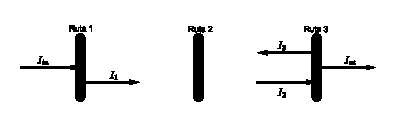
\includegraphics[scale=2]{images/tripleglazing.eps}
\caption{Visualisering av variabelnamnen använda vid härledning av reflektionsparametern för treglasfönster.}
\label{fig:tripleglazing}
\end{figure}

För en treglasruta gäller en något mer komplicerad annan reflektionsparameter. Betrakta figur \ref{fig:tripleglazing}. För $I_1$, den intensitet som släpps igenom första rutan, gäller att 

\begin{equation}
I_1=I_{in}\left( 1-a \right).
\end{equation}

På grund av en oändlig följd av reflektioner, även från den del av $I_3$ som passerar ruta 2 igen, blir $I_2 = \left( 1-a \right) I_1 \sum_{n=0}^{\infty} a^{2n} + a \left( 1-a \right)^2 I_3 \sum_{n=0}^{\infty} a^{2n}$. Men samtidigt måste också $I_3 = aI_2\sum_{n=0}^{\infty} a^{2n}$ vilket, om $I_2$ bryts ut, ger att

\begin{equation}
I_2 = \frac{\left( 1-a \right) I_1 \sum_{n=0}^{\infty} a^{2n}}{1-\left( 1-a \right)^2a^2\left(\sum_{n=0}^{\infty} a^{2n}\right)^2}.
\end{equation}

Detta tillsammans med det faktum att 

\begin{equation}
I_{ut} = \left( 1-a \right)I_2\sum_{n=0}^{\infty} a^{2n}
\end{equation}

ger, då dessa tre samband kombineras, att

\begin{equation}
I_{ut} = \frac{\left( 1-a \right)^3\left( \sum_{n=0}^{\infty} a^{2n}\right)^2}{1-\left( 1-a \right)^2a^2\left(\sum_{n=0}^{\infty} a^{2n}\right)^2}I_{in}.
\end{equation}

Notera nu att $\sum_{n=0}^{\infty} a^{2n} = \frac{1}{1-a^2}$ på grund av geometriska seriers egenskaper. Sätt in detta och förenkla så fås tillslut att

\begin{equation}
I_{ut} = \frac{\left( 1-a \right)^3}{\left(\left( 1-a^2\right)^2 - \left(1-a\right)^2 a^2\right)}I_{in} = 0,75 \cdot I_{in}
\end{equation}

då $a=0.1$.

\section{Värmeledning}
\label{sec:heatconduction}

Det pågår ständigt värmetransport från varma till kalla objekt. Konduktion, eller värmeledning, innebär att värmeenergi flödar genom ett material, utan att materialet i sig rör sig eller flyttar sig. Värmetransporten är proportionell mot temperaturskillnaden över konstruktionen. Konduktiviteten, eller värmeledningsförmågan, ofta betecknad $k$ inom fysiken eller $\lambda$ inom byggsektorn är en materialegenskap som beskriver hur snabbt en temperaturskillnad utjämnas genom konduktion i enheten $\unit{W~m^{-1}~K^{-1}}$. I denna rapport används den förstnämnda symbolen, $k$. För att bestämma $k$ för ett material utsätter man det för en temperaturskillnad och mäter den värmemängd som passerar genom materialet per tidsenhet. Generellt gäller att värmeflödet per ytenhet är $\mathbf{q} = - \unit[k \nabla T]{Wm^{-2}}$. Detta samband brukar kallas för Fouriers värmelag. I en dimension förenklas detta till

\begin{equation}\label{eq:conduction:fourier}\boxed{ \; \; \;
q_x = -k \frac{\mathrm{d}T}{\mathrm{d}x} \unit{Wm^{-2}}.
\; \; \; }
\end{equation}

Vid termisk jämvikt och homogent material kan detta utvecklas till

\begin{equation}
q_x = -\frac{k}{\mathrm{d}}\left( T_2-T_1\right) \unit{Wm^{-2}},
\end{equation}

där $d$ betecknar materialets tjocklek och $T_2$ samt $T_1$ är temperaturen i vardera änden av materialet. Begreppet U-värde kan nu införas och definieras som $U = \frac{k}{\mathrm{d}} \unit{Wm^{-2}K^{-1}}$, det vill säga $q_x = U\mathrm{d}T = U\left( T_2-T_1 \right)$. Även R-värdet introduceras och definieras som inversen av U-värdet, alltså $R=1/U \unit{m^2KW^{-1}}$. Observera att U- respektive R-värden endast kan användas vid termisk jämvikt, se härledningen nedan. Dessa två storheter är ofta användbara inom byggfysik och relaterade områden eftersom man med dem exempelvis kan jämföra olika väggars värmeledningsförmåga.

En schematisk bild över en vägg i en dimension som består av $n$ olika material kan ses i figur~\ref{fig:staticwallmethod:wall}. Med materialens värmeledningsförmåga, $k_i$, för $i=1,2\,,\,...\,,\,n$ samt längden på elementen, $d_i$, använder vi nu Fouriers värmeledningsekvation för att teckna värmeflödet och temperaturerna $T_i$, i punkterna mellan de olika delarna av väggen med randvillkoren $T_1 = T_H$ samt $T_{n+1} = T_L$.

\begin{figure}[hpbt]
\centering
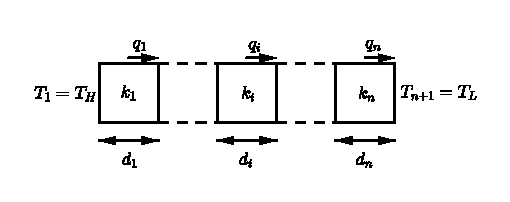
\includegraphics[scale=1.2]{images/wall.eps}
\caption{Schematisk bild över en vägg som består av $n$ olika element med olika
längd och värmeledningsförmåga.}\label{fig:staticwallmethod:wall}
\end{figure}

För varje del av väggen kan vi sätta upp ekvationer från Fouriers ekvation för värmeflöde. Vid termisk jämvikt blir flödet in i en del lika stort som flödet ut ur samma del vilket leder till att

\begin{equation}
\label{eq:staticwallmethod:rod}
q_i = -k_i\frac{T_{i+1}-T_{i}}{L_i} \, \Leftrightarrow \, \frac{L_i}{k_i}q_i = T_{i+1}-T_{i}
\end{equation}

Termisk jämvikt ger även att $q_1 = \, ... \, = q_i = \, ... \, = q_n$, vilket innebär att

\begin{equation}
\sum_{i=1}^n \frac{L_i}{k_i}q_i = q\sum_{i=1}^n \frac{L_i}{k_i} = q\sum_{i=1}^n R_i = \sum_{i=1}^n \left( T_{i}-T_{i+1} \right) = T_H - T_L 
\end{equation}

det vill säga

\begin{equation}
q R_\text{total} = T_H - T_L \Leftrightarrow q = U_\text{total} \left( T_H - T_L \right)
\end{equation}

där

\begin{equation}
U_\text{total} = \frac{1}{R_\text{total}} = \frac{1}{\sum_{i=1}^N R_i}.
\end{equation}

Värmeledningsförmågan, och därmed även R- samt U-värden, påverkas av materialets densitet, porositet, temperatur samt fuktighet. Fuktkorrigering görs ibland, enligt vissa framställda värden.

Utifrån Fouriers värmelag kan man härleda ytterligare ett viktigt samband, värmeledningsekvationen. Anta en infinitesimal volym, som varken utsätts för eller utför något arbete relativt omgivningen. Enligt grundläggande termodynamik kan då en godtyckligt liten förändring av värmeenergin (i $\unit{J m^{-3}}$) skrivas som $\mathrm{d}Q = c_p \rho \mathrm{d}T$.  I en dimension, över ett litet tidssteg $t-\mathrm{d}t< \tau < t+\mathrm{d}t$ och en liten sträcka $x-\mathrm{d}x < l < x+\mathrm{d}x$, fås att

\begin{equation}
\mathrm{d}E = c_p \rho \int_{x-\mathrm{d}x}^{x+\mathrm{d}x} \left[ T\left( l, t+\mathrm{d}t\right) - T\left( l, t-\mathrm{d}t\right)\right]dl = c_p \rho \int_{t-\mathrm{d}t}^{t+\mathrm{d}t} \int_{x-\mathrm{d}x}^{x+\mathrm{d}x} \frac{\partial T}{\partial \tau} \mathrm{d}l\mathrm{d}\tau
\end{equation}

Från Fouriers värmelag blir för samma förändring

\begin{equation}
\mathrm{d}E = k\int_{t-\mathrm{d}t}^{t+\mathrm{d}t} \left[ \frac{\partial T}{\partial x}\left( x + \mathrm{d}x, \tau \right) - \frac{\partial T}{\partial x}\left( x-\mathrm{d}x, \tau \right)\right]d\tau =  \int_{x-\mathrm{d}x}^{x+\mathrm{d}x} \frac{\partial}{\partial x} \left( k \int_{t-\mathrm{d}t}^{t+\mathrm{d}t} \frac{\partial T}{\partial x} \mathrm{d}\tau \right)\mathrm{d}l
\end{equation}

Kombinering av dessa och det faktum att det gäller för en godtycklig sträcka $\mathrm{d}l$ samt tid $\mathrm{d}\tau$, vilket innebär att integralen kan tas bort, ger att

\begin{equation}\label{eq:conduction:heateq}\boxed{ \; \; \;
c_p \rho \frac{\partial T}{\partial t} = \frac{\partial}{\partial x} \left( k \frac{\partial T}{\partial x} \right) \Leftrightarrow \frac{\partial T}{\partial t} = \alpha \Delta T
\; \; \; }
\end{equation}

där det andra sambandet gäller då $k$ är oberoende av $x$. Detta samband brukar kallas för värmeledningsekvationen.

\paragraph{Tröghet}
Det kan förefalla intuitivt att väderförändringar påverkar fastigheter, men hur mycket det spelar roll det egentligen? I det resonemanget spelar termen tröghet en betydande roll. Beroende på hur tjocka väggarna är, samt vilket material de är byggda av spelar de yttre omständigheterna olika stor roll. Trögheten i väggarna är således ett begrepp för hur lång tid det tar innan en väderförändring märks inomhus då yttre parametrarna ändrar sig. En stor tröghet bidrar till ett jämnare inomhusklimat då väggarna fungerar som lågpassfilter och dämpar svängningarna i temperaturen.

\section{Svartkroppsstrålning}
\label{sec:blackbody}

Alla objekt reflekterar, absorberar eller transmitterar ljus. De kroppar som varken 
reflekterar eller transmitterar något ljus utan absorberar $\unit[100]{\%}$ kallas konventionellt för svartkroppar. Detta är dock en teoretisk konstruktion då perfekta svartkroppar inte existerar men modellen kan ändå användas som en god modell i flera fysikaliska 
tillämpningar. Den energi som absorberats av kroppen strålas ut i form av svartkroppsstrålning vars 
frekvensspektrum bestäms av kroppens temperatur när kroppen är i termisk jämvikt med
 sin omgivning. Den totala utstrålade energin per tidsenhet fås ur Stefan-Boltzmanns lag
 
\begin{equation}
\label{eq:boltzmanslag}
\boxed{ \; \; \;
j^{\star} = \sigma T^{4}
\; \; \; }
\end{equation}

\noindent
där $\sigma$ är Stefan-Boltzmanns konstant som mäts i $\unit{W~m^{-2}~K^{-4}}$ och $T$ är kroppens temperatur vid termisk jämvikt.

\subsection{Härledning}
% av stefan-boltzmanns lag
% med hål i en låda
% kolla i termoboken
I en låda med fotoner kan den totala energin inne i lådan beskrivas som 
\begin{equation}
\label{eq:photonbox}
\frac{U}{V}=\frac{8\pi^5}{15}\frac{(kT)^4}{(hc)^3}
\end{equation}

där $U$ är  och $V$ är lådans volym. Ekvationen fås ur Plancks spektrum.\cite[ss.~301-302]{schroeder00} % Ev. förtydliga mer om vad som fås ur Plancks spektrum och vad U är.

Sedan görs ett litet hål i lådan, så att några av fotonerna kan slippa ut. Sannolikheten för att fotoner med kort respektive lång våglängd ska slippa ut är densamma som fördelningen mellan dem inne i lådan, eftersom de har samma hastighet.

Den totala mängden strålning som kommer ut kan då beräknas genom att tänka sig att 
de fotoner som når fram till hålet under en kort tidsperiod, $\mathrm{d}t$, alla befann sig
 på samma hemisfäriskt skal inne i lådan för en liten stund sedan, se figur \ref{fig:box}. Tjockleken på detta tänkta hemisfäriska skal är $c\mathrm{d}t$. Hemisfärens radie, $R$, beror givetvis på hur långt bakåt i tiden vi tittar.

\begin{figure}[hpbt]
\centering
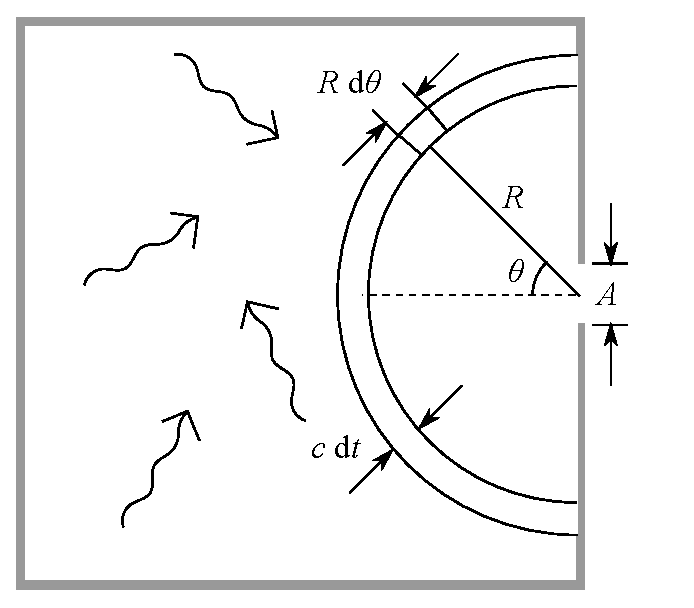
\includegraphics[height=5cm]{images/blackbody_box.eps}
\caption{\label{fig:box}{Fotonerna som lämnar lådan har en liten stund tidigare befunnit sig i samma hemisfär inne i lådan.}}
\end{figure}


Ett volymelement av det hemsfäriska skalet ges av
\begin{equation}
V=(R\mathrm{d}\theta) \times (R\sin\theta\mathrm{d}\phi) \times (c \mathrm{d}t).
\end{equation}

Energitätheten för fotonerna i volymelementet är således
\begin{equation}
E_\text{v.e.}=\frac{U}{V} c \mathrm{d}t R^2 \sin\theta \mathrm{d}\theta \mathrm{d}\phi.
\end{equation}

Men endast den andel av fotonerna som har rätt riktning kommer ut genom lådans öppning. Sannolikheten för att en foton har rätt riktning är
\begin{equation}
P(\text{rätt riktning})=\frac{A\cos\theta}{4\pi R^2}
\end{equation}

där A är hålets area. Den totala energin som strålar ut ur hålet från det lilla 
volymelementet är alltså 
\begin{equation}
\frac{A\cos\theta}{4\pi}\frac{U}{V} c\mathrm{d}t \sin\theta\mathrm{d}\theta \mathrm{d}\phi
\end{equation}

vilket ger en total energiutstrålning på
\begin{equation}
\frac{A}{4}\frac{U}{V}c \mathrm{d}t.
\end{equation}

Givetvis är utstrålningen beroende av både hålets area och tidsintervallet. Dividerar vi med dessa storheter får vi effekt per ytenhet, $j$,
\begin{equation}
j=\frac{c}{4}\frac{U}{V}. 
\end{equation}

Sätt in detta uttryck i ekvation~\eqref{eq:photonbox} så fås det vi känner som Stefan-Boltzmans lag,~\eqref{eq:boltzmanslag}
\begin{equation}
j=\frac{2\pi^5}{15}{(kT)^4}{h^3c^2}=\sigma T^4
\end{equation}

där $\sigma=\frac{2\pi^5k^4}{15h^3c^2}$ är Stefan-Boltzmans konstant.


\subsection{Strålning från omgivningen}
\label{sec:bb_sur}

\begin{figure}[hpbt]
\centering
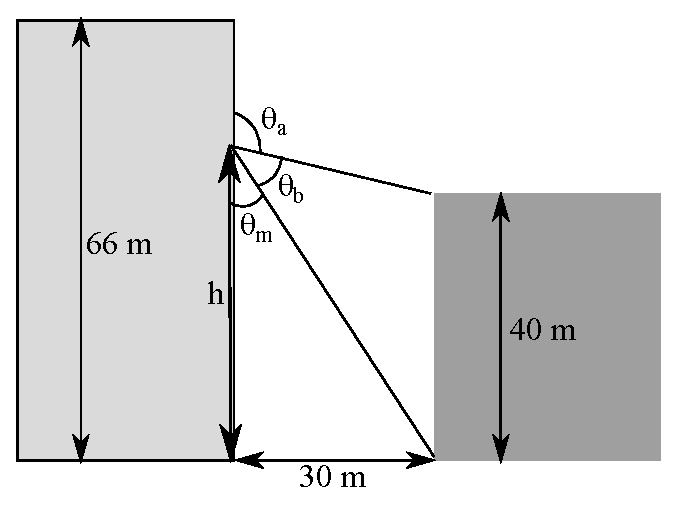
\includegraphics[height=4cm]{images/blackbody_surroundings.eps}
\caption{\label{fig:surroundings}{Den undersökta fastigheten på 
Wallerius\-gatan till vänster, och Johannebergs\-kyrkans församlings\-hem till höger. Den mot väggen instrålade svartkroppstrålningen kommer från olika källor. Här illustreras hur mycket av väggens omgivning som upptas mark, annan fastighet respektive atmosfären.}}
\end{figure}

För att uppskatta hur mycket svartkroppsstrålning som kommer mot väggen från olika 
delar av omgivningen sattes en enkel modell upp. Där antas att Johannebergskyrkans 
församlingshem ligger mitt emot vår undersökta fastighet på Walleriusgatan, att 
församlingshemmet ligger 30 meter bort och är 40 meter högt samt att det är det enda 
föremålet av betydande storlek i närheten, se figur~\ref{fig:surroundings}. För varje punkt
 på väggen beskrivs sedan hur stor andel av dess omgivning som upptas av marken, 
 församlingshemmet respektive himlen, eller atmosfären, med hjälp av ekvationerna

\begin{equation}
p_\text{gata}=\tan^{-1}(30/h)/180
\end{equation}

\begin{equation}
p_\text{byggnad}= \left\{
\begin{array}{rl}
\tan^{-1}(\frac{30}{h-40})/180 & \text{om } h > 40 \\
(\tan^{-1}(\frac{40-h}{30})+\tan^{-1}(\frac{h}{30}))/180^\circ & \text{om } h < 40 \\
\end{array} \right.
\end{equation}

\begin{equation}
p_\text{atmosfär}=1-p_\text{gata}-p_\text{byggnad}.
\end{equation}

Medelvärdet då $h$ går från 0 till 66 meter ger det genomsnittliga värdet för hur stor del av omgivningen som representeras av mark, annan fastighet och atmosfär för hela väggen. Detta ger resultatet att 26\% är gata, 36\% är 
 församlingshemmet och 38\% är atmosfären. Oftast antas allt som inte är atmosfären ha utomhustemperatur.

\cite{bb_atmosphere} ger atmosfärens temperatur genom en modifierad variant av Stephan-Boltzmans lag och att strålningen från atmosfären en klar dag kan beskrivas som 
\begin{equation}
I_\text{atmosfär}=\sigma\cdot T_\text{ute}^4(1-c \cdot e^{-d(273-T_\text{ute})^2})
\end{equation}
där $c=0,261$ och $d=7,77\cdot10^{-4}$ kommer ur statistiska data. En helt molnig dag är atmosfärens temperatur samma som utomhustemperaturen, $T_\text{ute}$, det vill säga $c=0$. Denna ekvation har fåtts ut statistiska data och visar sig stämma bra för hela världen\cite{bb_atmosphere}.
\section{Konvektion}
\label{section:convection}
I fasta ämnen går det utmärkt att approximera värmeflöde enbart med hjälp av värmeledningsekvationen. Detta håller dock ej lika bra för fluider, det vill säga material som deformeras då de utsätts för tryck. Under dessa förhållanden måste det tas hänsyn till konservation av massa, rörelsemängd och energi. I det följande kommer en homogen fluid betraktas. För att härleda giltiga differentialekvationer som beskriver en fluids rörelse används ofta sambandet

\begin{equation}
\label{eq:convection:reynolds}
\frac{dB}{dt} = \frac{d}{dt}\left( \int_{V} \frac{dB}{dm} \rho dV \right) + \int_{\partial V} \frac{dB}{dm} \rho \left( \mathbf{v} \cdot \mathbf{n} \right)dA,
\end{equation}

där $B$ är en godtycklig egenskap av fluiden, exempelvis dess rörelsemängd, V är den så kallade kontrollvolymen (omfattande ett godtyckligt valt område), $\partial V$ är denna kontrollvolyms rand, $\rho$ är fluidens densitet, $\mathbf{v}$ är fluidens hastighetsvektor och $\mathbf{n}$ är normalvektorn till randen. Detta samband benämns vanligen Reynolds transportteorem\footnote{För närmare beskrivning och härledning, se White, 2011 \cite{white11}}.

Sätt $B = m$ där $m$ är fluidens massa (oberoende av tiden) och låt $V$ vara en tidsoberoende volym. Ett uttryck för masskonservering erhålls:

\begin{equation}
\label{eq:convection:masscon}
0 = \int_V \frac{\partial \rho}{\partial t} dV + \int_{\partial V} \rho \left( \mathbf{v} \cdot \mathbf{n} \right) dA
\end{equation}

Första termen i detta uttryck beskriver förändringar i densiteten inom kontrollvolymen medan andra termen omfattar alla flöden in och ut genom kontrollvolymens rand. För masskonservering krävs alltså att summan av dessa termer ska vara noll.

Den andra termen kan skrivas om med hjälp av Gauss sat (även kallad divergenssatsen),

\begin{equation}
\label{eq:convection:gauss}
\int_{\partial V} \rho \left( \mathbf{v} \cdot \mathbf{n} \right) dA = \int_V \nabla \cdot \rho \mathbf{v} dV
\end{equation}

\begin{figure}[hpbt]
\centering
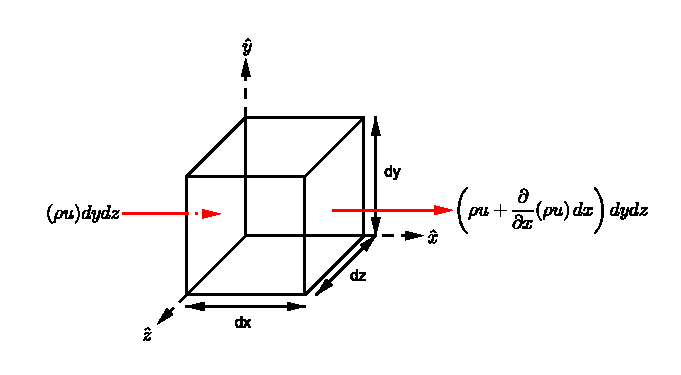
\includegraphics[scale=1]{images/massflowcube.eps}
\caption{\label{fig:massflowcube} Infinitesimal kontrollvolym för derivering av bevaranderelationer, här med massflödet exemplifierat}
\end{figure}

Betrakta nu en infinitesimal kontrollvolym som den i figur \ref{fig:massflowcube}. Integralerna över V ersätts med den infinitesimala volymen $dxdydz$ och \eqref{eq:convection:masscon} reduceras till

\begin{equation}
\label{eq:convection:massconinf}
0 = \left( \frac{\partial \rho}{\partial t} + \nabla \cdot \rho \mathbf{v}\right) dxdydz
\end{equation}

vilket, om $dxdydz$ förkortas bort, kan förenklas som

\begin{equation}
\label{eq:convection:continuity}
\boxed{ \; \; \;
0 = \frac{\partial \rho}{\partial t} + \nabla \cdot \left( \rho \mathbf{v} \right) 
\; \; \; }
\end{equation}

Om inkompressibilitet antas ($\rho$ = konstant) reduceras denna ekvation ytterligare till

\begin{equation}
\label{eq:convection:continuityinc}
\nabla \cdot \mathbf{v} = 0
\end{equation}

Detta är kontinuitetsekvationen för inkompressibla fluider.

Betrakta åter \eqref{eq:convection:reynolds} och sätt nu $B = m\mathbf{v}$. På samma vis som kontinuitetsekvationen \eqref{eq:convection:continuityinc} härleddes, fås för det infinitesimala volymelementet i figur sambandet

\begin{eqnarray}
\label{eq:convection:linear}
\sum \mathbf{F} & = & \frac{\partial}{\partial t} \left( \int_V \rho\mathbf{v} dV \right) + \int_{\partial V} \mathbf{v}\rho\left( \mathbf{v} \cdot \mathbf{n}\right)dV \nonumber \\
& = &\left(\frac{\partial}{\partial t} \left( \rho\mathbf{v} \right) + \nabla \cdot \left( \mathbf{v} \rho \mathbf{v}\right)\right)dxdydz \nonumber\\
& = &\left( \frac{\partial}{\partial t} \left( \rho\mathbf{v} \right) + \mathbf{v}\left(\nabla\cdot\rho\mathbf{v}\right) + \left(\rho\mathbf{v} \cdot \nabla\right) \mathbf{v}\right) dxdydz
\end{eqnarray}

ty enligt Newtons andra lag är tidsderivatan av rörelsemängden $m\mathbf{v}$ lika med summan av alla krafter som verkar på kroppen. $\dot{m}_i$ betecknar här massflödet $\rho\mathbf{v}_i\cdot\mathbf{A}_i$.

Det sista högerledet kan skrivas om som

\begin{equation}
\left( \mathbf{v}\left[ \frac{\partial \rho}{\partial t} + \nabla\cdot \rho \mathbf{v}\right] + \rho\left[ \frac{\partial \mathbf{v}}{\partial t} + u\frac{\partial\mathbf{v}}{\partial x} + v\frac{\partial\mathbf{v}}{\partial y} + w\frac{\partial\mathbf{v}}{\partial z} \right]\right)dxdydz.
\end{equation}

Första termen inom hakparentes är kontinuitetsekvationen \eqref{eq:convection:continuity} och går alltså bort.

Därmed reduceras \eqref{eq:convection:linear} till

\begin{equation}
\label{eq:convection:linearfinal}
\sum \mathbf{F} = \rho \left( \frac{\partial \mathbf{v}}{\partial t} + \mathbf{v}\cdot \nabla\mathbf{v} \right)dxdydz.
\end{equation}

Summan av de på volymen verkande krafterna måste nu utvecklas. Dessa krafter uppstår på grund av gravitation, tryck och viskositet. Andra krafter, såsom från elektromagnetiska fält, kan i sammanhanget anses vara försumbara. Gravitationskraften $\mathbf{F}_g$ beskrivs för den infinitesimala volymen med $\rho \mathbf{g} dxdydz = \rho g dxdydz \hat{z}$. Tryckkraften $\mathbf{F}_p$, i sin tur, ges av tryckgradienten $-\nabla \left( p \right) dxdydz$. Viskösa kraften $\mathbf{F}_{visc}$ är lite besvärligare att sammanställa. Anta att volymen är en Newtonsk fluid, det vill säga stresstensorn $\tau$ är linjärt proportionell mot hastighetsgradienten $\nabla\mathbf{v}$ med proportionaltitetskonstanten $\mu$, $\tau = \mu \nabla \mathbf{v}$. Den viskösa kraften verkande på kroppen blir då $\mathbf{F}_{visc} = \mu\Delta\mathbf{v}dxdydz$.

% Skriv om till integralrelationer och använd gauss sats, därefter infinitesimal volym

Vi har alltså ekvationssystemet

\begin{equation}
\label{eq:convection:momentum}
\addtolength{\fboxsep}{10pt} 
\boxed{ 
\begin{split} 
\rho\left(\frac{\partial u}{\partial t} + \mathbf{v}\cdot \nabla u\right) & = -\frac{\partial p}{\partial x} + \mu\Delta u\\
\rho\left(\frac{\partial v}{\partial t} + \mathbf{v}\cdot \nabla v\right) & = -\frac{\partial p}{\partial y} + \mu\Delta v\\
\rho\left(\frac{\partial w}{\partial t} + \mathbf{v}\cdot \nabla w\right) & = -\rho g -\frac{\partial p}{\partial z} + \mu\Delta w  
\end{split} 
} 
\end{equation}

% Energirelationen

Slutligen sätts i \ref{eq:convection:reynolds} $B=E$ för att söka ett uttryck för energins bevarande. Med antagandet att volymen inte utför något arbete blir $E = Q$, där $Q$ betecknar värmeenergin, och på samma vis som i avsnitt\ref{sec:heatconduction} blir $Q = c_p \rho dT$, vilket ger följande:

\begin{eqnarray}
\label{reynoldsenergyone}
\frac{dQ}{dt} & = & \frac{\partial}{\partial t} \int_V \frac{dQ}{dm}\rho dV + \int_{\partial V}\frac{dQ}{dm}\rho \mathbf{v} \cdot \mathbf{n} dA \nonumber\\
& = & \frac{\partial}{\partial t} \int_V c_p T \rho dV + \int_{\partial V} c_p T \rho \mathbf{v} \cdot \mathbf{n} dA \nonumber\\
& = & \left(\frac{\partial}{\partial t} \left( c_p T \rho \right) + \nabla\cdot c_p T \rho \mathbf{v}\right) dxdydz \nonumber\\
& = & c_p \rho \left( \frac{\partial T}{\partial t} + \mathbf{v}\cdot \nabla T\right)
\end{eqnarray}

Sista steget följer av att kontinuitetsekvationen bryts ut som i fallet med rörelsemängdsekvationen. För att utveckla vänsterledet betraktas återigen en infinetisemal volym såsom i figur \ref{fig:massflowcube}. Värmeenergiflödet in i volymen i x-led ges av $q_x dy dz$ medan utflödet ges av $\left[ q_x + \frac{\partial}{\partial x} \left( q_x\right)dx\right]dydz$ och analogt för y- respektive z-led. Totala ökningen av värmeenergi i kuben ges alltså av utflödet subtraherat från inflödet, vilket innebär att

\begin{equation}
\frac{dQ}{dt} = - \nabla \cdot \mathbf{q} dxdydz.
\end{equation}

$\mathbf{q}$ fås från Fouriers värmelag (se avsnitt \ref{sec:heatconduction}) vilket ger att

\begin{equation}
\label{reynoldsenergytwo}
\frac{dQ}{dt} = \left( - \nabla \cdot \left( -k \nabla T \right) \right)dxdydz
\end{equation}

och detta i sin tur leder till resultatet

\begin{equation}
\label{eq:convection:energy}\boxed{ \; \; \;
\nabla \cdot \left( k \nabla T \right) = c_p \rho \left( \frac{\partial T}{\partial t} + \mathbf{v}\cdot \nabla T\right)
\; \; \;}
\end{equation}

För homogena inkompressibla fluider i två dimensioner gäller alltså ekvationerna
\eqref{eq:convection:continuityinc}, \eqref{eq:convection:momentum} samt \eqref{eq:convection:energy}.

\subsection{Vindens konvektionskoefficient}

Då vinden blåser kommer en del värmeenergi överföras via konvektion, men istället för att lösa den invecklade konvektions-diffussionsekvationen används ofta något som kallas för vindens konvektionskoefficient, betecknat med $h$. I analogi med Fouriers värmelag, ekvation \ref{eq:conduction:fourier}, skrivs

\begin{equation}\boxed{ \; \; \;
q = hdT = h\left( T_{wall} - T_{\infty}\right).
\; \; \;}\end{equation}

där h alltså ka jämföras med det ovan härledda U-värdet. 

Denna konvektionskoefficient beskrivs ofta av en ekvation anpassad till empiriska resultat, och ett stort antal experiment har genomförts för att bestämma parametern, även om en helhetsbild saknas i dagsläget.

Vid fri (naturlig) konvektion, det vill säga då vinden är försumbar och luftcirkulationen följer av stigande varm luft, brukar h fås till mellan 2 och $\unit{25}{Wm^{-2}K^{-2}}$. Vid forcerad konduktion, det vill säga då vinden inte är försumbar, kan h variera från 25 till $\unit{250}{Wm^{-2}K^{-2}}$. \cite{ASHRAE09}

Traditionellt används ofta något som kallas för Nusselt-Jürges korrelation vid beräkning av konvektionskoefficienten, som lyder

\begin{equation}
h = 5.678 \left( a + b \left( \frac{965.42}{T_{out}}\left(|\mathbf{v}_{wind}\times \mathbf{n}|\right) \right)^c \right)
\end{equation}

där $\mathbf{n}$ betecknar väggens normalvektor, och a, b samt c beror på väggens ytegenskaper. För en skrovlig yta med $|\mathbf{v}_{vind}\times \mathbf{n}| < \unit{4.88}{ms^{-1}}$ fås att $a=1.09$, $b=0.23$ samt $c=1$, medan starkare vind ger $a=0$, $b=0.53$ samt $c=0.78$.

En mängd andra samband mellan konvektionskoefficienten och vindhastigheten har härletts, både teoritiskt och empiriskt, på grund av dess starka beroende av byggnadens ytegenskaper och area, men av anledningar som diskuteras i avsnitt \ref{sec:errors}.\cite{palyvos08}

% Skapa graf över T och v beroende

\subsection{Boussinesq approximation}

För flytkraftsdrivet flöde kan det vara lämpligt att använda sig av
Boussinesq approximation. Denna säger att det enda som påverkar trycket är
tyngdaccelerationen. Genom detta är det möjligt att sätta upp uttryck för densiteten
och tryckderivatorna enligt ekvationerna \eqref{eq:convection:density}
och \eqref{eq:convection:pressurez}. Här är
$\beta$ den volymetriska expansionskonstanten och
$T_0$ temperaturen som råder vid referensdensiteten $\rho_0$.

\begin{equation}
\label{eq:convection:density}
\rho = \rho_0[1-\beta(T-T_0)]
\end{equation}

\begin{equation}
\label{eq:convection:pressurez}
\frac{\partial p}{\partial z} = -\rho_0g
\end{equation}



\subsection{Finita element av inkompressibel fluid}

För att lösa Navier-Stokes ekvationer kan lämpligen en datormodell användas.
Här består denna modell av ett system uppsatt med Galerkins metod.
I denna lösning så begränsar vi dock oss till att enbart behandla statiska flöden
vilket genomförs genom att sätta alla tidsderivator till noll.

För att hantera trycket i \eqref{eq:convection:continuity}-\eqref{eq:convection:energy} används den tidigare nämnda Boussinesq approximation
samt penalty metoden för att göra hastighetsvektorn källfri och uppfylla
kontinuitetsekvationen. Det finns således inget direkt behov av att räkna ut trycket.
Vid användning av många sorters elementtyper som inte uppfyller Babuska-Brezzikriteriet
är detta dessutom nödvändigt då det annars kan bildas oönskade trycknoder. 
En annan möjlighet är att välja divergensfria element. \cite{babuska1973}\cite{segal2011}

Genom penaltymetoden beskrives här trycket som $p$ enligt ekvation
\eqref{eq:femconvection:penalty}. Här är $p_s$ någon form av idealt statiskt
tryck som är önskat. Detta tryck följer Boussinesq approximation. Med dessa
idealiseringar kan differentialekvationerna sättas upp igen. \cite{heinrich88}\cite{taylor79}
Som kan ses så leder den godtyckliga penaltyparametern $\lambda$ till att justera trycket
om hastighetsfältets divergens ej är identiskt noll. I viss litteratur anges 
det att penaltyparametern skall vara i storleksordningen $10^7$ men att den
är väldigt applikationsberoende. En för liten vald penaltyparameter leder till att
trycket inte elimineras. Andra problem uppstår vid en för stor parameter. Ekvationssystemet
kan bli svårlöst och få stabilitetsproblem när parametern blir
för stor i jämförelse med de andra delarna i differentialekvationen.\cite{reddy93}\cite{roy05}\cite{basak04}\cite{segal2011}

\begin{equation}
\label{eq:femconvection:penalty}
p = p_s - \lambda\nabla\cdot\mathbf{v}
\end{equation}

\noindent
Fortsatt skall trycket deriveras med avseende på de rumsliga variablerna vilket möjliggör
att eliminera trycket från differentialekvationerna. Dessa deriveringar kan ses i ekvation
\eqref{eq:femconvection:partx} samt \eqref{eq:femconvection:partz}. Notera att det statiska trycket
$p_s$ ej beror på $x$ vilket resulterar i att derivatan är noll.

\begin{equation}
\label{eq:femconvection:partx}
\frac{\partial p}{\partial x} = \frac{\partial p_s}{\partial x} -
\frac{\partial}{\partial x} \lambda\nabla\cdot\mathbf{v} = -
\frac{\partial}{\partial x} \lambda\nabla\cdot\mathbf{v}
\end{equation}

\begin{equation}
\label{eq:femconvection:partz}
\frac{\partial p}{\partial z} = \frac{\partial p_s}{\partial z} -
\frac{\partial}{\partial z} \lambda\nabla\cdot\mathbf{v} =
-g\rho_0 - \frac{\partial}{\partial z} \lambda\nabla\cdot\mathbf{v}
\end{equation}

\noindent
Detta förs in i momentekvationerna vilket ger ekvationerna \eqref{eq:femconvection:u} -
\eqref{eq:femconvection:T}. Här är det ekvationssystem som syftar att lösas.

\begin{equation}
\label{eq:femconvection:u}
\mathbf{v}\cdot\nabla u =
\frac{\lambda}{\rho_0}\nabla\cdot\mathbf{v} +
\nu\Delta u
\end{equation}

\begin{equation}
\label{eq:femconvection:w}
\mathbf{v}\cdot\nabla w =
\frac{\lambda}{\rho_0}\nabla\cdot\mathbf{v} + \nu\Delta w +g\beta(T-T_0)
\end{equation}

\begin{equation}
\label{eq:femconvection:T}
\mathbf{v}\cdot\nabla T = \alpha\Delta T
\end{equation}

\subsubsection{Svag formulering}

En finita elementlösning med Galerkins metod kräver att problemet reduceras till
ett ekvivalent variationsproblem. Här söks $T\in\Phi$, $u\in\Phi$ och
$w\in\Phi$ som uppfyller ekvation \eqref{eq:femconvection:variation}. Här
betecknar brackets skalärprodukt, $\mathbf{L}$ är differentialoperatorn
som betecknar systemet av differentialekvationer som $\mathbf{L}(T,u,w) = 0$.
$\Phi$ är rummet av alla testfunktioner $\phi$ som är kontinuerliga i
definitionsmängden $\Omega$ samt vars derivator är bitvis kontinuerliga på randen
$/Gamma$. De måste även vara $L^2$ integrabla.

\begin{equation*}
\label{eq:femconvection:variation}
\langle \mathbf{L}(T,u,w), \phi \rangle = 0\mbox{,  } \forall \phi \in \Phi
\end{equation*}


\section{Optimering med Newton-Raphsons metod}

När ett ekvationssystem är ickelinjärt kan ej exakta metoder som Gausseliminering användas
för ekvationslösning. Detta stötte vi till exempel på vid finita elementlösningen
av Navier-Stokes ekvationer i avsnitt \ref{sec:femconvection}.
I dessa fall måste approximativa optimeringsmetoder utnyttjas. En sådan
metod är Newton-Raphsons metod. Denna bygger på trunkerad Taylorutveckling 
av en funktion för att linjarisera ett ickelinjärt ekvationssystem
$\mathbf{f}(\mathbf{x}) = 0$
vilket kan ses i ekvation \eqref{eq:newtonsmethod:taylor}. Här är
$\mathbf{J}_f(\mathbf{x})$ jacobianen för $\mathbf{f}(\mathbf{x})$. 

\begin{equation}
\label{eq:newtonsmethod:taylor}
\mathbf{f}(\mathbf{x} + \Delta\mathbf{x}) \approx \mathbf{f}(\mathbf{x}) +
\mathbf{J}_f(\mathbf{x})\Delta\mathbf{x}
\end{equation}

\noindent
Principen går ut på att algoritmen upprepat gissar nya lösningar där de
nya lösningarna följer den negativa jacobianen. Till en början är en god initial gissning
$\mathbf{x}_0$ ett kriterie för att Newton-Raphson skall konvergera. Därefter så beräknas
funktionsvärdet $\mathbf{f}(\mathbf{x}_0)$ samt jacobianen $\mathbf{J}_f(\mathbf{x}_0)$.
Dessa används för att beräkna nästa gissning genom att lösa
\eqref{eq:newtonsmethod:guess} och beräkna nästa $\mathbf{x}$ med
\eqref{eq:newtonsmethod:nextx}. \cite{heath2002}

\begin{equation}
\label{eq:newtonsmethod:guess}
\mathbf{J}_f(\mathbf{x}_n)\Delta\mathbf{x}_n = -\mathbf{f}(\mathbf{x_n})
\end{equation}

\begin{equation}
\label{eq:newtonsmethod:nextx}
\mathbf{x}_{n+1} = \mathbf{x}_n + \Delta\mathbf{x}_n
\end{equation}

\noindent
Itereringen bör avbrytas då ett maxantal itereringar har uppnåtts och funktionen
ej har konvergerat alternativt när felet är tillräckligt litet. En av styrkorna 
med denna algoritm är dess kvadratiska konvergens mot enkelrötter. \cite{ympa95}
En svaghet med Newton-Raphson är att det i många fall ej är möjligt att analytiskt beräkna
jacobianen. Istället måste andra algoritmer untnyttjas som till exempel finita differensmetoden
för beräkning av jacobianen. Omvägar som denna bidrar till att lösningsprocessen blir mycket
mer omständig och processorintensiv. 

\subsection{Konvergens samt konvergenskriterier}

För att enklare förstå några problem som kan uppstå med Newton-Raphsons metod kan det vara lämpligt
att repetera beviset av dess kvadratiska konvergens. Definiera en funktion $f(x)$ enligt \eqref{eq:newtonproof}.
Antag att den roten $f(x) = 0$ existerar för $x = \alpha$.

\begin{align}
f: & \mathbb{R} \to \mathbb{R} \nonumber \\
   & x \mapsto f(x) \label{eq:newtonproof}
\end{align}

\noindent
Härnäst genomförs en taylorutveckling av funktionen $f(x)$ i ekvation \eqref{eq:newtonprooftaylor}.
Den kvadratiska termen är här Lagranges restterm med parametern $\xi_n \in [\alpha, x_n]$.

\begin{equation}
\label{eq:newtonprooftaylor}
f(\alpha) = f(x_n) + f^\prime(x_n)(x_n-\alpha) + \frac{f^{\prime\prime}(\xi_n)}{2}(x_n-\alpha)^2
\end{equation}

\noindent
Nu kan förstaderivatan av $f(x_n)$ divideras över samt $f(\alpha)$ är känt att vara noll.
Efter detta identifieras $f(x_n)/f^\prime(x_n) = x_n-x_{n+1}$ och ersätts. Slutligen så ses
det i ekvation \eqref{eq:newtonqed} att $x_{n+1}-\alpha \propto (x_{n}-\alpha)^2$.

\begin{equation}
0 = \frac{f(x_n)}{f^\prime(x_n)} + \alpha - x_n + \frac{f^{\prime\prime}(\xi_n)}{2f^\prime(x_n)}(x_n-\alpha)^2
\Rightarrow
\end{equation}

\begin{equation}
\label{eq:newtonqed}
x_{n-1} - \alpha = - \frac{f^{\prime\prime}(\xi_n)}{2f^\prime(x_n)}(x_n-\alpha)^2 
\end{equation}

\noindent
För att ovanstående bevis ska gälla så måste andraderivatan vara uppåt begränsad, förstaderivatan får ej
vara noll och den högre ordningens derivator får ej vara av stor betydelse för funktionens uppträdande
nära roten $f(x) = 0$. Rent praktiskt innebär detta att en god gissning är essentiell för att få
konvergens i metoden. Även med en god gissning så kan problem uppstå om derivatan av funktionen
förändras snabbt i omgivningen av $x$. Detta kan resultera i både att nästa gissning ligger för långt
bort och för nära. Det förstnämnda problemet innebär att metoden hoppar över roten vilket till och med
kan innebära att metoden divergerar. Det andra problemet är mindre allvarligt då det endast innebär 
att metoden förlorar sin kvadratiska konvergens.

\subsection{Förbättrad Newton-Raphson}

En metod för att hantera att metoden hoppar över rötter är att i varje steg försöka minimera $|f(x_{n+1})|$.
Rent praktiskt innbär detta att vi väljer en konstant $0 \le k_n \le 1$ och genomför ett modifierat
Newtonsteg enligt ekvation \eqref{eq:newtonmodified}.

\begin{equation}
\label{eq:newtonmodified}
x_{n+1} = x_n - k_n\frac{f(x_n)}{f^\prime(x_n)}
\end{equation}

\noindent
För att identifiera det optimala valet av $k_n$ kan godtycklig linjesökningsalgoritm användas. Ett val av metod
är att behandla det analytiskt för att göra metoden mindre processorintensiv. En ny funktion definieras
enligt ekvation \eqref{eq:newtong} med $\Delta x_n = f(x_n)/f^\prime(x_n)$.

\begin{equation}
\label{eq:newtong}
g(k_n) = f(x_n- k_n\Delta x_n)
\end{equation}

\noindent
I ekvation \eqref{eq:newtongmin} deriveras funktionen med avseende på $k_n$ i punkten $k_n=0$
och kedjeregeln används för att skriva om uttrycket till något som är användbart.

\begin{align}
\frac{\partial g(k_n)}{\partial k_n}\,\bigg|_{k_n=0} & = 
\left(\frac{\partial g(k_n)}{\partial (k_n\Delta x_n)}
\frac{\partial k_n \Delta x_n}{\partial k_n}\right)\,\bigg|_{k_n=0} = \nonumber \\
x_n \frac{\partial f(x_n- k_n\Delta x_n)}{\partial (k_n\Delta x_n)}\,\bigg|_{k_n=0} & = 
-\Delta x_n f^\prime(x_n) = - f(x_n)
\label{eq:newtongmin}
\end{align}

\noindent
Ett förslag på algoritm är nu att i varje iterationssteg först beräkna det fulla newtonsteget motsvarande $k_n=1$.
Är då $f(x_{n+1}) < f(x_n)$ så kan steget godtagas. Stämmer inte detta så beräkas derivatan av $g(k_n)$ och
funktionen $g(k_n)$ ansätts vara ett polynom av andra ordningen enligt ekvation \eqref{eq:newtonfit}.

\begin{equation}
\label{eq:newtonfit}
g(k_n) = ak^2_n + bk_n + c
\end{equation}

\noindent
Nu kan de kända värdena $g(0)$, $g(1)$ samt $g^\prime(0)$ användas för att lösa ut koefficienterna i polynomet.
Dessa kan slutligen användas för att beräkna derivatan av $g(k_n)$ för att hitta dess minimum och således
hitta den optimala parametern $k_n$.

\noindent
Om denna metod skall användas för att lösa ett ekvationssystem istället för en realvärd funktion i en dimension
så behövs något mått sättas upp. Problemet som önskas att lösas är $\mathbf{F}(\mathbf{x}) = 0$.
Funktionen som skall minimeras kan då med fördel väljas till $f(\mathbf{x}) = \mathbf{F}(\mathbf{x})^2/2$.
På ett analogt sätt ovan så beräknas derivatan av funktionen $g(k)$ till ekvation \eqref{eq:newtonvecg}.\cite{fortran77}

\begin{equation}
\label{eq:newtonvecg}
g_n^\prime(0) = - \mathbf{F}(\mathbf{x_n})^2 \le 0
\end{equation}

\noindent
För att hitta roten $\mathbf{F}(\mathbf{x}) = 0$ så ansätts som ovan ett polynom där koefficienterna beräknas.
Som kan ses så existerar det ett $k_n$ så att $\mathbf{F}(\mathbf{x}_{n+1}) \le \mathbf{F}(\mathbf{x}_n)$ ty
$g^\prime(0) \le 0$ och enbart noll om roten redan är funnen.


\section{Naturkonstanter för luft}

Vid olika tryck, fuktighet, temperatur och annat väder som påverkar. Luft består av 78,1\% kväve och 21,0\% syre (mer exakt http://en.wikipedia.org/wiki/Air\#Composition)

\subsection{Termisk diffusivitet}
In heat transfer analysis, thermal diffusivity is the thermal conductivity divided by density and specific heat capacity at constant pressure. It has the SI unit of $m^2/s$. The formula is:

\begin{equation}
\alpha = {k \over {\rho c_p}}
\end{equation}

where
\begin{itemize}
   \item[] k is thermal conductivity, $\unit{W/(m·K)}$
   \item[] $\rho$ is density, $\unit{kg/m^3}$
   \item[] $c_p$ is specific heat capacity, $\unit{J/(kg·K)}$
\end{itemize}

Air: $\unit[1.9\cdot10^{-5}]{m/s^2}$

Källor:\\
http://www.electronics-cooling.com/2007/08/thermal-diffusivity/\\
http://en.wikipedia.org/wiki/Thermal\_diffusivity\\

\subsubsection{Termisk konduktivitet}
The property of a material's ability to conduct heat. Unit: W/(m·K).

\subsubsection{Desitet}

https://www.brisbanehotairballooning.com.au/faqs/education/116-calculate-air-density.html

Gäller så länge ideala gaslagen gäller vilket den gör vid lufttryck. Källa?




\subsubsection{Specifik värmekapacitivitet}
kan approximeras med konstanten 1.005 kJ/(kg·K (källa: http://www.engineeringtoolbox.com/air-properties-d\_156.html) (för torr luft).

\subsection{Volymetriska expantionskoefficienten}

\subsection{Kinematiska viskositeten}

\subsection{Andra funderingare}
Fråga någon på Geofysik, Klimat, t.ex. någon här: http://www.gvc.gu.se/Forskning/klimat/stadsklimat/gucg/people/


\end{document}



\section{Ekvivalent temperatur}

Kort sagt är ekvivalent temperatur det värde man ersätter utomhustemperaturen för att ta 
hänsyn till fler väderparametrar än just utomhustemperaturen i styrningen av en 
klimatanläggning.

Att bara ta hänsyn till utomhustemperaturen vid injustering av klimatsystem är enkelt. 
Tyvärr är det lite för enkelt för att det ska bli riktigt bra, eftersom flera andra 
väderparametrar, främst sol och vind, värmer och kyler fastigheten i olika grad. I resultatdelen i den här rapporten visas det mer exakt hur mycket.

De energiflöden i väggen som orsakas av väderleken summeras med energiflödet 
som uppkommer av utomhustemperaturen. Dessa jämförs sedan med energiflöden från 
olika utomhustemperaturer, utan övrig väderpåverkan, och den temperatur som ger 
samma energiflöde kallas ekvivalent temperatur. Denna kan sedan ersätta 
utomhustemperaturen som indata till klimatsystemet och ge ett jämnare inomhusklimat.

% är det bra
% varför används det


% Tidigare text:
%Antag att det bara finns ett sorts väder, där temperaturen är den enda variabeln. Det
% skulle innebära att man kan hänföra hur mycket energi som går åt för att värma upp 
% någonting direkt till utetemperaturen. Det finns oändligt antal olika vädertyper, och fler 
% parametrar måste tas i beaktning då man räknar ut hur mycket energi som måste tillföras
%  huset. En ekvivalent temperatur för en viss vädertyp skulle således motsvara den 
%  temperaturen, i ett optimalt klimat, som kräver tillförsel av samma energimängd för att 
%  upprätthålla efterfrågat klimat.
